\section{Redes neuronales aplicadas a imágenes}
Desde el punto de vista del aprendizaje automático, se ha abordado con múltiples herramientas y modelos el problema de la clasificación automática de imágenes. Los avances sucedidos en el campo, también han tenido un efecto en dentro de la clasificación automática de imágenes. Dentro de esos avances, hay que destacar la aparición de la técnica ``Back Propagation'' que hizo posible el entrenamiento de redes neuronales de gran profundidad. Este tipo de modelos, que tratan de imitar el comportamiento de un cerebro, han producido un gran avance en este campo.\\

Las redes neuronales convolucionales, dan un paso más allá, obteniendo grandes resultados en los tipos de datos en el que la información de un punto está especialmente vinculada a la de sus vecinos, como pasa en las imágenes.\\
 
Dada la gran utilidad e importancia de este modelo concreto para la tarea, se definirán sus componentes, y se realizará una pequeña comparación con las redes neuronales usuales para tratar de mostrar sus ventajas.\\

\subsection{Definición de neurona artificial}

Por ser un modelo bioinspirado, primero es necesario conocer el funcionamiento básico de una neurona natural. Las neuronas son la unidad básica de nuestro cerebro. En él, podemos encontrar aproximadamente 86 mil millones de neuronas, conectadas en entre ellas mediante $10^{14}$ y $10^{15}$ sinapsis. En la figura \ref{partes-neurona} podemos ver las diferentes partes de una neurona. Las dendritas funcionan como la entrada de información por medio de la sinapsis con otras neuronas. El impulso es transmitido al núcleo de la neurona y tras esto, la señal de salida es emitida por el axión hacia otras neuronas. Estudiaremos el proceso paso a paso definiendo en cada momento el equivalente de la neurona artificial, para llegar a la fórmula final que la representa.\\

\begin{figure}
\begin{center}

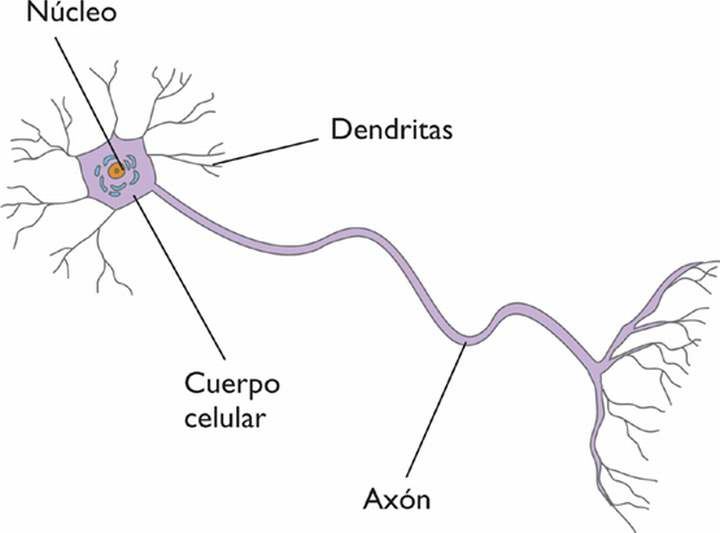
\includegraphics[scale=0.35]{img/partes_neurona.jpg}
\end{center}

\caption{Partes de una neurona.}
\label{NN}
\end{figure}

La entrada de una neurona artificial será por tanto un conjunto de valores $\left\lbrace x_1,x_2,\ldots,x_N\right\rbrace$ con $x_n \in \mathbb{R}$, para $n = 1,\ldots,N$. Las dendritas de la neurona, pueden ser excitadas, facilitando la activación de la neurona o inhibidas, dificultándolo. Para simular esto, se añaden una serie de pesos $\left\lbrace w_1,w_2,\ldots,w_N\right\rbrace$ con $w_n \in \mathbb{R}$, para $n = 1,\ldots,N$, que multiplicarán a las entradas y un valor adicional $b \in \mathbb{R}$, llamado bías, que representa la facilidad de la neurona para activarse. Los pesos y el bías son de una gran importancia para el aprendizaje de la red, pues una vez definida la red, son los únicos elementos que se puede aprender. Esto simula también el aprendizaje humano, que se realiza mediante el cambio de comportamiento de las neuronas y de como se afectan unas a otras, haciendo que puedan pasar a inhibir, excitar o incluso a desaparecer el enlace por carecer de importancia, simulado en las redes neuronales como un peso 0.\\

Tras esto núcleo de la neurona combina las entradas que recibe. En el modelo de la neurona artificial, esta combinación se realiza mediante la suma de las entradas, es decir: $$\sum^N_{n=1} x_n w_n + b. $$

La activación de la neurona es un proceso brusco. Si pasa de un umbral, se activa. Este proceso se modela en la práctica con una gran cantidad de funciones. La discusión sobre que función elegir tiene más que ver con el entrenamiento de las redes en su conjunto que con el funcionamiento de la neurona. La única restricción que se le impone es que sea diferenciable.\\

Juntando todos los elementos, representamos una neurona artificial mediante la siguiente ecuación:

$$f\left( \sum^N_{n=1} x_n w_n + b. \right).$$

\subsection{Redes Neuronales Artificiales}

Siguiendo con el modelo inspirado en el cerebro, el siguiente paso son las redes neuronales. Tras ver el modelo de una neurona, y el comportamiento de una neurona real, podemos apreciar que la capacidad de aprendizaje de este elemento es relativamente pequeño. La verdadera capacidad reside en la unión de las neuronas en conjuntos interconectados de las mismas, llamadas redes neuronales.\\
 
Las redes neuronales artificiales simplifican esta realidad, incluyendo las siguientes restricciones:
\begin{itemize}
\item \textbf{Organización por capas:} Las redes neuronales artificiales se organizan por capas. Es decir, la entrada de la capa i, son las salidas de la capa i-1, y las salidas de la capa i, serán las entradas de la capa i+1. Esta organización tan forzada y artificial no se cumple así en los cerebros reales. 
\item \textbf{No hay retroalimentación:} Las neuronas no pueden conectarse a capas anteriores. Esta restricción se incluye se podría encajar dentro de la anterior, pero tiene importancia propia. La retroalimentación sí sucede en la realidad, y se cree que es importante para el funcionamiento de un cerebro. Existen modelos que incluyen este fenómeno, pero no son tan populares como este modelo simplificado. 
\end{itemize}

El modelo de las redes neuronales artificiales es bastante claro tras estas restricciones con respecto a las redes de neuronas naturales. Se definen de 3 tipos de capas distintas:
\begin{itemize}
\item \textbf{Capa de entrada:} Red sin ningún tipo de pesos ni función de activación. Pasan directamente los datos de entrada a la primera capa oculta.
\item \textbf{Capa oculta:} Toman los datos de la capa anterior, utiliza los pesos de cada neurona para combinarlos, calculan la función de activación y pasan su salida a la siguiente capa. Normalmente, todas las capas ocultas de la red tienen el mismo tipo de función de activación.
\item \textbf{Capa de salida:} Salida de la red. Funcionamiento similar a una capa oculta, con la diferencia que la función de activación puede ser diferente al resto de la red. La elección de la función de activación depende del problema de la red, para permitir dar una salida acorde al problema.
\end{itemize}

\begin{figure}
\begin{center}

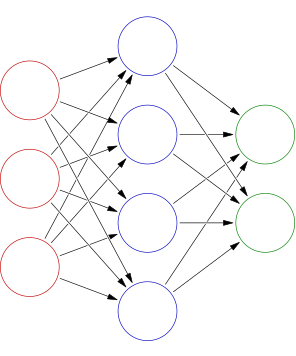
\includegraphics[scale=0.5]{img/NN.png}
\end{center}

\caption{Red neuronal de dos capas.}
\label{NN}
\end{figure}

Una red neuronal consta de una primera capa de entrada, seguida por varias capas ocultas, terminando en una capa de salida. En la figura \ref{NN} podemos ver un ejemplo de red neuronal artificial. Se puede denotar la arquitectura de la red por el número de capas ocultas y de salida que tenga. Se hace así al obviar dentro de la arquitectura la capa de entrada, por no tener pesos en comparación a las otras dos.\\

\subsubsection{Propiedades}

Estas redes son muy generales. Las redes neuronales artificiales de dos capas son aproximadores universales. Es decir, una red neuronal de dos capas puede aproximar uniformemente cualquier función continua en un dominio de entrada compacto, con una precisión arbitraria dada, si tiene suficientes neuronas en la capa oculta\cite{Cybenco}\cite{Hornik}.\\

Sin embargo, las redes de una capas oculta no han conseguido ser un éxito a nivel práctico. El resultado teórico no nos informa del número de neuronas que tenemos en la capa intermedia y aún suponiendo que conocida una función, pudiéramos saber el número de neuronas necesaria, en el marco del aprendizaje automático no conocemos la función que queremos aproximar. Por tanto, pese a conocer esta propiedad, no la podemos utilizar al no saber si el tamaño de la capa será suficiente.\\

Por el otro, ya vimos que los modelos que tienen una gran capacidad para aprender pueden también sobreaprender. Una segunda mirada a la propiedad podría ser que tiene una capacidad infinita de aprender. Esto lleva a pensar que si la capa intermedia tiene demasiadas neuronas, sobreaprenderá, lo cual puede ser factor negativo.\\


\subsection{Entrenamiento de una red neuronal}

Vamos a estudiar el desarrollo seguido en \cite{Bishop:2006:PRM:1162264}. Hasta ahora, hemos visto las redes neuronales como una familia de funciones paramétricas no lineal. Evidentemente, nuestro objetivo es obtener los mejores parámetros para ajustar la red y que consiga la mejor aproximación al problema planteado. Es equivalente conseguir la mejor aproximación a reducir una medida de error. Tomaremos como medida del error la suma de los errores cuadráticos. Siendo $y(x,w)$ el resultado de la ejecución de la red al dato de entrada $x$, usando los pesos $w$, siendo ${x_n}$ el conjunto de datos de entrenamiento, con $n=1\ldots N$,junto con los vectores objetivo ${t_n}$, la función de suma del error cuadrático que usaremos, para unos pesos $w$, es:

\[
\ E(W)= \frac{1}{2} \sum_{n=1}^N \parallel y(x_n,w)-t_n \parallel^2 .
\]

En la práctica, la no linealidad de la red neuronal hace que $E(w)$ sea no convexo, luego pueden aparecer mínimos locales, lo que complica la tarea de buscar el mínimo del error.\\

\subsubsection{Uso del gradiente}

Como sabemos, el gradiente de una función $f(x)$, $\nabla f(x)$, tiene la propiedad de indicar la dirección de máximo crecimiento en el punto $x$. Esto es equivalente a que $-\nabla f(x)$ sea la dirección de máximo decrecimiento de la función en el punto $x$. Esta propiedad se usa para el entrenamiento de las redes neuronales y en muchos otros modelos habituales dentro del aprendizaje automático.\\

El acercamiento más sencillo a esta técnica es elegir la actualización de los pesos de la red dando un pequeño paso en la dirección del gradiente negativo. Siendo $w^{(\tau)}$ los pesos en la iteración $\tau$ y siendo $\eta>0$ el ratio de aprendizaje, la actualización de los pesos se realiza mediante

\[
\ w^{(\tau +1)}=w^{(\tau)}+\eta \nabla E(w^{(\tau)}) .
\]

Después de la actualización, se vuelve a repetir el proceso con los nuevos pesos. Notar que cada actualización requiere el procesado de todos los datos del conjunto de entrenamiento. Los métodos que hacen esto se conocen como métodos ``batch''. Existen métodos de este tipo más eficientes, que además aseguran descender siempre en cada paso que dan. En el modelo anterior que pese a avanzar en la dirección de máximo decrecimiento no está asegurado dicho descenso, pues al ser fijo el ratio de aprendizaje $\eta$ puede hacernos avanzar más de lo deseado en esa dirección, permitiendo crecer el error tras una actualización.\\

Existe también una versión on-line, que se suele llamar optimización secuencial, del método del gradiente descendiente que ha conseguido grandes resultados en el entrenamiento de redes neuronales con grandes bases de datos. Sea $E_n(w)$ el error en la muestra $n$. El método de actualización de la optimización secuencial sería

\[
\ w^{(\tau +1)}=w^{(\tau)}+\eta \nabla E_n(w^{(\tau)}) .
\]

El proceso sigue tomando imágenes de manera secuencial o haciendo un muestreo aleatorio con reemplazo. También existen enfoques intermedios, que son muy utilizados y que siguen esta misma idea.\\

Este tipo de versiones del gradiente descendiente donde no se usa todos los datos de entrenamiento en cada iteración, si no un subconjunto de los mismos, se llaman gradiente descendiente estocástico. Entre sus ventajas, destacar por un lado el cálculo de la actualización usando un subconjunto de los datos de entrada es más rápido que el mismo cálculo con la base de datos de entrenamiento entera, lo que es muy importante con conjuntos de entrenamiento que pueden llegar a contener millones de datos. Además, el gradiente obtenido en el proceso estocástico puede sacar el proceso de mínimos locales, pues al no usar todos los datos, el gradiente puede no ser 0. Por último, maneja mejor la redundancia de datos. En el caso extremo de tomar un conjunto de entrenamiento y duplicar su tamaño, duplicando uno a uno todos los datos, el método del gradiente descendiente estocástico apenas se vería afectado, mientras que el gradiente descendiente usual tardaría en realizar una actualización el doble de tiempo.\\

Destacar que el método de actualización de los pesos utilizado para explicar estos conceptos es muy simple. Existen técnicas que, basandose en el mismo concepto de desplazarse en la dirección del gradiente, introducen mejoras como ratio de aprendizaje descendente, ratio de aprendizaje variable o tener en cuenta los movimientos anteriores, es decir su inercia.\\ 

\subsubsection{Backpropagation}

Hemos visto que, sin importar el tipo de entrenamiento que elijamos, el proceso se basa en calcular el gradiente de una función. Esto no supone ningún tipo de problema, pues las funciones utilizadas para la activación de las neuronas artificiales tienen derivadas fácilmente calculables. El problema es la eficiencia de dicha operación, pues tanto la derivada usual mediante el uso de la regla de la cadena, como las aproximaciones usando diferencias finitas son muy lentas cuando la red crece en número de capas y número de pesos. Hablaremos más de esto cuando entremos a fondo en la eficiencia.\\

Para salvar este obstáculo, se diseñó una nueva técnica para el cálculo del gradiente, conocido como ``backpropagation''. Destacar que esta palabra solo hace referencia al hecho de propagar los errores por la red hacia atrás, es decir del final de la red al principio, aunque es común utilizarla para hablar del proceso completo de cálculo del gradiente. Nos centraremos en calcular $\nabla E_n(w)$.\\
 
 \todo[inline,color=red]{Cuentas de la backpropagation}
 
En el fondo, todo este proceso no es más que una simple aplicación de la regla de la cadena. Su potencial se encuentra principalmente en su eficiencia.\\

Lo primero que tenemos que destacar es que simplemente evaluar una red ya es un proceso que no es muy eficiente. Para una red grande, lo normal es que el número de pesos $W$ sea muchas veces mayor que el número de neuronas. Por lo tanto, el mayor tiempo empleado durante la ejecución de la evaluación de la red es en las operaciones de productos y sumas entre los pesos y los valores de la capa anterior, permitiéndonos considerar el calculo de la función de activación como un overhead. Por tanto, el tiempo de ejecución dependerá linealmente de $W$, luego el coste computacional de la operación es $O(W)$.\\

La alternativa a la técnica backpropagation es el uso de la aproximación de las diferentes derivadas por medio de diferencias finitas. Esta aproximación la podemos expresar mediante

\[
\ \frac{\delta E_n}{\delta w_{ij}} = \frac{E_n(w_{ij}+\epsilon) - E_n(w_{ij})}{\epsilon} +O(\epsilon),\qquad\textrm{con }\epsilon>0.
\]

Para obtener una buena aproximación, tenemos que acercar $\epsilon$ todo lo posible a 0 pero sin llegar a tener problemas de inestabilidades numéricas. Pero pese a poder obtener buenos resultados con esta aproximación o con algunas de coste similar y mayor precisión, no es eficiente. Tendríamos que repetir el cálculo de la aproximación una vez por cada peso de la red, y un simple cálculo de $E_n(w)$ ya es una operación $O(W)$. Luego el cálculo del gradiente utilizando diferencias finitas para aproximar las derivadas es una operación de coste computacional $O(W^2)$.\\

Aún así, este método es muy simple de programar. Por lo tanto tiene su lugar en el desarrollo de redes neuronales, para poder comprobar que el método del cálculo del gradiente, mucho más complicado y más propicio a fallos de programación, funciona correctamente.\\

\subsection{Deep Learning}

El proceso habitual en el mundo del aprendizaje automático estaba limitado en su habilidad para procesar datos naturales directamente. Durante mucho tiempo hizo falta un minucioso proceso para diseñar un conjunto de características que transformaran los datos de entrada en una representación aceptable para el sistema de aprendizaje\cite{lecun-nature}.\\

Se llama aprendizaje de la representación a un conjunto de métodos que automáticamente tratan de reconocer estas representaciones optimas para los posteriores métodos de aprendizaje. Deep Learning se encaja dentro de este tipo de métodos. En él, la composición de varias capas de funciones simples pero no lineales, hace que cada capa obtenga una representación más compleja y de más alto nivel. Con la composición de muchas de estas capas, se pueden aprender funciones muy muy complejas. El aspecto fundamental del Deep Learning es que las características obtenidas no han sido diseñadas por un ingeniero, se aprenden automáticamente siguiendo un procedimiento de caracter general.\\
 
Esta técnica ha conseguido grandes avances en el mundo de la inteligencia artificial. Es extremadamente buena encontrando estructuras complejas dentro de los datos de alta dimensionalidad, haciéndola especialmente útil para muchos dominios. En concreto, es una de las partes fundamentales de los grandes resultados que se obtienen en el campo de la clasificación de imágenes. Evidentemente, este problema encaja dentro del caso anterior: datos con una gran dimensionalidad y características complejas que eran necesarias diseñar por los ingenieros.\\

Pero la aplicación directa de estos métodos, pese a ser efectiva, puede tener algunos problemas con respecto a las imágenes. Imaginemos el problema de clasificar imágenes relativamente pequeñas, de 32x32 píxeles RGB. Tendríamos entonces 3072 datos de entrada. Por cada neurona de la primera capa, necesitaríamos 3073 pesos. Es fácil ver lo rápido que puede escalar el número de pesos al aumentar el tamaño de la red en un espacio de datos tan complejo.\\

En esa visión, sin embargo, se obvian características importantes de las imágenes, que permiten que existan modelos diferentes de redes neuronales mejor adaptadas al problema. Las redes neuronales convolucionales que introdujo el investigador Yann Lecun \cite{lecun-89e}\cite{lecun-98} tratan de explotar estas características, consiguiendo grandes resultados en su aplicación en la práctica.\\ 

\subsection{Redes neuronales convolucionales}

Consideremos el problema del reconocimiento de números escritos a mano. Cada entrada es una imagen, que contiene un conjunto de valores de píxeles, y cuya salida esperada es la distribución de probabilidad sobre los diez tipos de números. Sabemos que la identidad de los números es invariante a escalados, pequeñas rotaciones y algunos tipos de deformaciones. Una red neuronal, con la suficiente cantidad de ejemplos, podría aprender esas invarianzas.\\

Pero sin embargo, este acercamiento ignora una propiedad fundamental de las imágenes. Los píxeles más cercanos están mucho más relacionados que los píxeles lejanos. En Visión por Computador, el uso de esta propiedad es muy normal, extrayendo propiedades locales de subregiones de la imagen. Dicha información local puede ser mezclada en etapas posteriores para detectar características de nivel superior, obteniendo finalmente una visión general de la imagen en su conjunto. Además las características locales que son útiles en una región es muy probable que también lo sea en otras, por ejemplo si el objeto esta desplazado.\\

Estas ideas se incorporan en las redes neuronales convolucionales mediante 3 aspectos: campo de entrada local, compartir pesos y submuestrear. En la capa de convolución, las neuronas se organizan en serie planos. Las neuronas de cada plano sólo tienen una pequeña ventana de entrada y además, todas las neuronas de un plano están obligadas a tener los mismos pesos. Si pensamos en las neuronas de una capa como detectores de características, podemos ver que tratan de extraer la misma característica pero a diferentes partes de la imagen. Debido a compartir pesos, la evaluación de una capa de este tipo de redes es equivalente a una convolución de la imagen con un kernel que dependería de los pesos de la capa. Como normalmente necesitamos detectar más de una propiedad para construir un modelo, lo normal es tener varios planos dentro de cada capa de convolución. Cada uno de estos planos contará con su propio conjunto de pesos, sirviendo cada capa para detectar una característica distinta.\\

La salida de la capa de convolución son la entrada de la capa de submuestreo. Se crean el mismo número de planos que en la capa de convolución. Para cada plano, se divide en pequeñas ventanas no solapadas y se genera el plano tras el submuestreo eligiendo uno de los valores de la ventana, normalmente el mayor. Este tipo de capas se utiliza para ir reduciendo poco a poco el tamaño de la red, ayudando a mejorar la velocidad de una ejecución de la red y reduciendo el número de parámetros, ayudando a un aprendizaje más rápido y controlando también el sobreentrenamiento.

\begin{figure}
\begin{center}

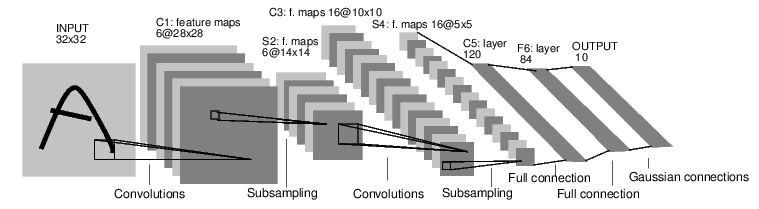
\includegraphics[scale=0.5]{img/lenet5.png}
\end{center}

\caption{Arquitectura de LeNet-5.}
\label{Lenet}
\end{figure}

En la figura \ref{Lenet} encontramos una representación visual de la red neuronal convolucional ``LeNet-5'', utilizada para clasificar dígitos. Se puede ver que en las capas de convolución (por ejemplo C1) encontramos diferentes planos. Cada plano calcula algún tipo de característica, y por tanto, todas las neuronas de cada plano comparten pesos. Además podemos ver otras características usuales de las redes neuronales convolucionales como el uso de los campos de entrada locales y el uso de submuestreo. La arquitectura aquí definida suele ser además la más usual, donde encontramos una repetición de capas de convolución y submuestreo hasta llegar a una serie de capas totalmente conectadas que acaban en la capa de salida.\\

Este tipo de modelos ha conseguido un gran éxito al ser aplicados a imágenes, demostrando su utilidad en varias bases de datos estándares de imágenes, convirtiéndose en el estado del arte de este tema.\\
%\subsection{Comparativa de redes neuronales}
